%% Seção 10: A Linguagem como Ferramenta de Diagnóstico, Intervenção e Transformação

\chapter{A Linguagem como Ferramenta de Diagnóstico, Intervenção e Transformação}

\epigrafe{O inconsciente é estruturado como uma linguagem.}{Jacques Lacan}

\textbf{10.} A linguagem é uma ferramenta central no diagnóstico, intervenção e transformação terapêutica, permitindo ao paciente reconstruir sua subjetividade e alcançar a autonomia.

\section{Linguagem como reflexo do estado interno}

\textbf{10.1} A linguagem reflete o estado interno do paciente, servindo como ferramenta diagnóstica para identificar disfunções cognitivas e emocionais.

\begin{tese}
Se a linguagem expressa os estados cognitivos e emocionais, então padrões de coerência ou fragmentação verbal podem diagnosticar desordens mentais.
\end{tese}

\begin{hipotese}[title=Hipótese 10.1.1 (Condicional)]
Se analisamos a linguagem do paciente, então podemos identificar sinais de desorganização mental ou emocional.
\end{hipotese}

\begin{referencia}[title=Referência a Bleuler]
Eugen Bleuler cunhou o termo ``esquizofrenia'' e destacou a importância das associações verbais e da linguagem no diagnóstico de distúrbios mentais.
\end{referencia}

\begin{aforismo}
Nas palavras desordenadas, revela-se a mente em desequilíbrio.
\end{aforismo}

\section{Reestruturação verbal como ferramenta terapêutica}

\textbf{10.2} A reestruturação verbal atua como ferramenta terapêutica ativa, reorganizando o pensamento e promovendo a integração interna.

\begin{tese}
Se a linguagem organiza o pensamento, então a reestruturação verbal pode ser usada como uma ferramenta terapêutica ativa.
\end{tese}

\begin{referencia}[title=Referência a Aaron Beck]
A Terapia Cognitiva utiliza a reestruturação cognitiva, onde a modificação dos pensamentos negativos automáticos é fundamental para a mudança emocional.
\end{referencia}

\begin{aforismo}
Na fala reordenada, a mente encontra seu novo equilíbrio.
\end{aforismo}

\section{Análise da fala como monitoramento terapêutico}

\textbf{10.3} A análise da fala serve como medida contínua de monitoramento terapêutico, refletindo o progresso ou retrocesso emocional do paciente.

\begin{tese}
Se a linguagem reflete tanto as disfunções quanto o progresso interno, então pode ser usada para monitorar o andamento terapêutico.
\end{tese}

\begin{referencia}[title=Referência a Melanie Klein]
A análise das comunicações verbais e não verbais é essencial para compreender os processos inconscientes em terapia.
\end{referencia}

\begin{aforismo}
Cada palavra dita ao longo do caminho é um marco do progresso interno.
\end{aforismo}

\section{O terapeuta e a linguagem como guia}

\textbf{10.4} O terapeuta utiliza a linguagem como ferramenta para guiar o paciente na reestruturação interna, influenciando positivamente seu processo de cura.

\begin{tese}
Se a linguagem pode ser tanto um reflexo quanto um meio de reorganização, então o terapeuta pode usá-la ativamente para promover mudanças internas.
\end{tese}

\begin{referencia}[title=Referência a Milton Erickson]
O uso estratégico da linguagem hipnótica para acessar o inconsciente e promover mudanças terapêuticas.
\end{referencia}

\begin{aforismo}
O terapeuta que escolhe bem suas palavras, escolhe o caminho certo para guiar a mente do paciente.
\end{aforismo}

\section{Reformulação verbal e transformação da subjetividade}

\textbf{10.5} A reformulação verbal pelo paciente transforma sua subjetividade, permitindo a reconstrução de sua identidade e promoção da autonomia.

\begin{tese}
Se a linguagem é uma ferramenta de intervenção, então a forma como o paciente reformula seus pensamentos através da fala pode transformar sua subjetividade.
\end{tese}

\begin{referencia}[title=Referência a Jacques Lacan]
A linguagem como estruturante do inconsciente; o sujeito é constituído no e pelo discurso.
\end{referencia}

\begin{aforismo}
Refazer o discurso é refazer o eu.
\end{aforismo}

%% DIAGRAMA DA SEÇÃO 10
\section*{Diagrama Representativo: Sistema Tripartite de Diagnóstico, Intervenção e Transformação}

\begin{center}
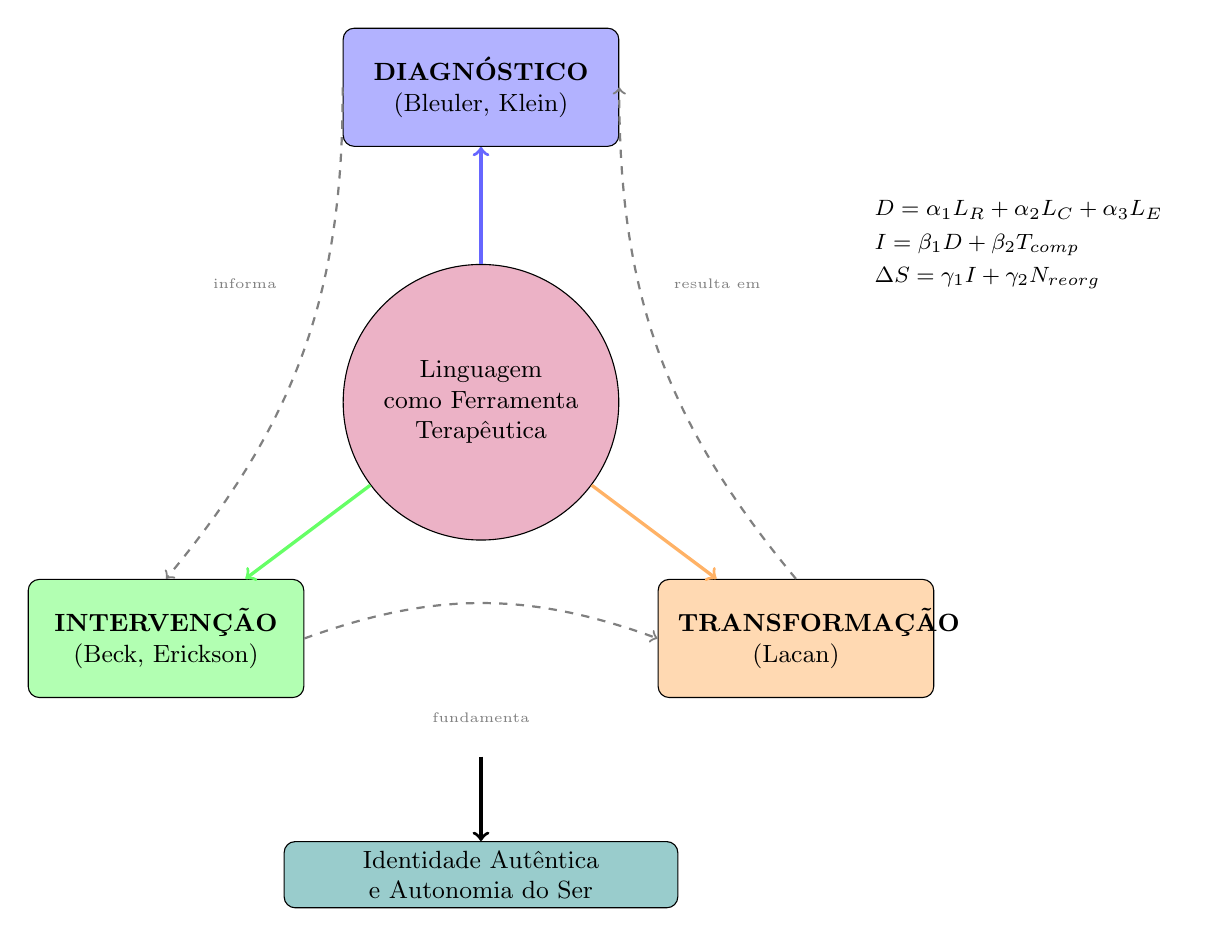
\begin{tikzpicture}[scale=1, every node/.style={font=\small}]
    % Linguagem no centro
    \node[draw, circle, fill=purple!30, minimum size=3.5cm, text width=2.5cm, align=center] (ling) at (0,0) {Linguagem\\como Ferramenta\\Terapêutica};

    % Três eixos
    \node[draw, rounded corners, fill=blue!30, minimum width=3.5cm, minimum height=1.5cm, text width=3cm, align=center] (diag) at (0,4) {\textbf{DIAGNÓSTICO}\\(Bleuler, Klein)};
    \node[draw, rounded corners, fill=green!30, minimum width=3.5cm, minimum height=1.5cm, text width=3cm, align=center] (inter) at (-4,-3) {\textbf{INTERVENÇÃO}\\(Beck, Erickson)};
    \node[draw, rounded corners, fill=orange!30, minimum width=3.5cm, minimum height=1.5cm, text width=3cm, align=center] (trans) at (4,-3) {\textbf{TRANSFORMAÇÃO}\\(Lacan)};

    % Setas do ciclo
    \draw[very thick, ->, blue!60] (ling) -- (diag);
    \draw[very thick, ->, green!60] (ling) -- (inter);
    \draw[very thick, ->, orange!60] (ling) -- (trans);

    % Ciclo entre os três
    \draw[thick, ->, gray, dashed] (diag.west) to[bend left=20] (inter.north);
    \draw[thick, ->, gray, dashed] (inter.east) to[bend left=20] (trans.west);
    \draw[thick, ->, gray, dashed] (trans.north) to[bend left=20] (diag.east);

    % Labels no ciclo
    \node[font=\tiny, gray] at (-3,1.5) {informa};
    \node[font=\tiny, gray] at (0,-4) {fundamenta};
    \node[font=\tiny, gray] at (3,1.5) {resulta em};

    % Resultado
    \node[draw, rounded corners, fill=teal!40, minimum width=5cm, text width=4.5cm, align=center] (result) at (0,-6) {Identidade Autêntica\\e Autonomia do Ser};
    \draw[very thick, ->] (0,-4.5) -- (result);

    % Fórmulas
    \node[font=\footnotesize, text width=4cm, align=left] at (7,2) {
        $D = \alpha_1 L_R + \alpha_2 L_C + \alpha_3 L_E$\\[0.3em]
        $I = \beta_1 D + \beta_2 T_{comp}$\\[0.3em]
        $\Delta S = \gamma_1 I + \gamma_2 N_{reorg}$
    };
\end{tikzpicture}
\end{center}

\subsection*{Modelo Matemático do Processo Terapêutico Integrado}

O processo terapêutico integrado pode ser representado como um sistema de equações:

\textbf{Diagnóstico:}
\begin{equation}
D = \alpha_1 L_R + \alpha_2 L_C + \alpha_3 L_E
\end{equation}

\textbf{Intervenção:}
\begin{equation}
I = \beta_1 D + \beta_2 T_{comp} + \beta_3 P_{eng}
\end{equation}

\textbf{Transformação:}
\begin{equation}
\Delta S = \gamma_1 I + \gamma_2 N_{reorg} + \gamma_3 \int I(t) \, dt
\end{equation}

Onde $L_R$, $L_C$, $L_E$ representam aspectos reflexivos, cognitivos e emocionais da linguagem; $T_{comp}$ é a competência terapêutica; $P_{eng}$ é o engajamento do paciente; $N_{reorg}$ é a reorganização narrativa; e $\Delta S$ é a mudança na subjetividade.

\begin{sintese}[title=Síntese Final da Seção 10]
A linguagem é uma ferramenta central no diagnóstico, intervenção e transformação terapêutica. Conforme Bleuler, a análise da linguagem permite identificar disfunções cognitivas e emocionais. A reestruturação verbal atua diretamente na reorganização do pensamento, alinhando-se com as abordagens de Aaron Beck e a Terapia Cognitiva. A análise contínua da fala, como proposto por Melanie Klein, serve para monitorar o progresso terapêutico.

O terapeuta utiliza a linguagem de forma estratégica para influenciar positivamente o processo de cura, seguindo os princípios de Milton Erickson. A reformulação verbal pelo paciente transforma sua subjetividade, em consonância com as ideias de Lacan sobre a linguagem e o inconsciente. Assim, a linguagem é o meio pelo qual a mente se revela, se organiza e se transforma, permitindo ao paciente reconstruir sua identidade e alcançar a autonomia do ser.
\end{sintese}

\nextpage
